\subsection{Der Zylinderresonator (Teilchen im unendlich hohen Potentialtopf)}

Schallwellen, die sich in einem abgeschlossenen zylinderförmigen Resonator befinden, können stehende Wellen ausbilden.
Voraussetzung hierfür ist die Resonanzbedingung

\begin{equation}
  L = n \lambda/2 = nc/(2f) .
\end{equation}

Dabei ist $L$ die Länge des Zylinders, $\lambda$ die Wellenlänge, $f$ die Frequenz und $c$ die Schallgeschwindigkeit im Medium
(hier in Luft). $n$ ist die Zahl der entsprechenden Mode.

Schallwellen können mit Hilfe des Drucks beschrieben werden. Ihre Wellengleichung lautet damit

\begin{equation}
  \Delta p(r,t) - \frac{1}{c^2} \frac{\partial^2 p(r,t)}{\partial t^2} = 0 .
  \label{eq:wellengl}
\end{equation}

Da sich in dem Zylinder nur longitudinale Wellen entlang der Symmetrieachse (hier: in $x$-Richtung) ausbreiten,
folgt ein eindimensionaler Lösungsansatz:

\begin{equation}
  p(x) = p_0 \text{cos}(kx)
\end{equation}

mit k = n\pi/L. Dies folgt aus den Randbedingungen

\begin{equation}
  \frac{\partial p(0)}{\partial x} = \frac{\partial p(L)}{\partial x} = 0 .
\end{equation}

Die Dispersionsrelation für Schallwellen lautet somit

\begin{equation}
  \omega(k) = ck = cn\frac{\pi}{L} .
\end{equation}

Solche stehenden Wellen im Zylinderresonator stellen ein klassisches Analogon zu quantenmechanischen Wellen in einem
unendlich hohen Potentialtopf dar.

Die quantenmechanische Darstellung erfolgt durch die Schrödingergleichung mit Wellenfunktion $\psi(x,t)$:

\begin{equation}
  i\hbar\frac{\partial\psi(x,t)}{\partial t}=-\frac{\hbar^2}{2m}\Delta\psi(x,t) + V(x)\psi(x,t) .
\end{equation}

Innerhalb des Kastenpotentials ($|x| < L/2$) gilt jedoch $V(x) = 0$. Außerhalb davon gilt $V(x) = \infty$.
$L$ bezeichnet die Länge des Kastens und $\hbar$ das reduzierte planck'sche Wirkungsquantum. Mit Hilfe eines Separationsansatzes
$\psi(x,t) = \phi(x)T(t)$ kann eine zeitunabhängige Lösung der Schrödingergleichung gefunden werden:

\begin{equation}
  \phi(x) = A \text{sin}(kx)
\end{equation}

mit k = n\pi/L. Dies folgt wieder aus den Randbedingungen: $\psi(0,t) = \psi(L,t) = 0$.

Damit ergibt sich die Dispersionsrelation für das quantenmechanische Kastenpotential zu

\begin{equation}
  E = \hbar \omega = \frac{\hbar^2 k^2}{2m}   \omega(k) = \frac{\hbar k^2}{2m}.
\end{equation}

bzw.

\begin{equation}
  \omega(k) = \frac{\hbar k^2}{2m}.
\end{equation}

\subsection{Der Kugelresonator (Wasserstoffatom)}

Auch im Kugelresonator können die Schallwellen mit Hilfe der Wellengleichung \ref{eq:wellengl} beschrieben werden.
Durch Abseparieren der Zeit $(p(r,t) = p(r)$cos$(\omega t))$ ergibt sich aus \ref{eq:wellengl} die Helmholtzgleichung:

\begin{equation}
  \Delta p(\vec{r}) + \frac{\omega^2}{c^2}p(\vec{r}) = 0 .
\end{equation}

Weiterhin können Radial- und Winkelanteil separiert werden, sodass $p(r,\theta,\phi) = R(r) Y_{ml}(\theta,\phi)$. Dabei
wir der Radialanteil durch die sogenannten Besselfunktionen beschrieben und der Winkelanteil durch die Kugelflächenfunktionen.

Für das Wasserstoffatom lautet die Schrödingergleichung

\begin{equation}
  E\psi(\vec{r})=-\frac{\hbar^2}{2m}\Delta\psi(\vec{r})-\frac{1}{4\pi\varepsilon_0}\frac{e^2}{r}\psi(\vec{r}) ,
\end{equation}

mit dem Coulombschen Potential und der Elementarladung $e$. Auch hier ist wieder eine Separation
in Radial- und Winkelanteil sinnvoll: $\psi(r,\theta,\phi) = R_{nl}(r) Y_{lm}(\theta,\phi)$.
Der Radialanteil wird in diesem Fall durch Legendre-Polynome beschrieben.
Hierbei sind $n, l$ und $m$ Quantenzahlen, die den Zustand eines Elektrons charakterisieren. $n$ ist die Hauptquantenzahl, welche
die Schale beschreibt, in der sich das Elektron befindet. $l$ beschreibt die Form des Orbitals, hängt mit dem Bahndrehimpuls
zusammen und nennt sich Nebenquantenzahl. Der Buchstabe $m$ ist die magnetische Quantenzahl und bezeichnet die Neigung des
Bahndrehimpulses im Raum.

Des Weiteren gibt es noch die sogenannte Spinquantenzahl, welche die Spinrichtung der Elektronen angibt (Spin-Up oder Spin-Down).

Die Energieeigenwerte des Wasserstoffatoms sind

\begin{equation}
  E_n = -E_{Ry} \frac{1}{n^2} .
\end{equation}

Dabei ist $E_{Ry}$ die Rydbergenergie. Aufgrund der Kugelsymmetrie sind die Energien in $m$ entartet.

\subsection{Das Wasserstoffmolekül}

Die Schrödingergleichung für ein Wasserstoffmolekül kann näherungsweise mit

\begin{equation}
  E\phi(\vec{r})=-\frac{\hbar^2}{2m}\Delta\phi(\vec{r})-\frac{1}{4\pi\varepsilon_0}\frac{e^2}{r_1}\frac{e^2}{r_2}\phi(\vec{r})
\end{equation}

beschrieben werden, wobei die Kerndynamik vernachlässigt wird. $r_1$ und $r_2$ sind die Abstände der Elektronen zum jeweils dazu
gehörenden Kern.
Aufgrund von Superposition können die beiden Ortswellenfunktionen $\Phi_1$ und $\Phi_2$ der beiden Elektronen addiert werden,
sodass sich zwei mögliche Wellenfunktionen für das Wasserstoffmolekül ergeben:

\begin{equation}
  \Phi^+(\vec{r}) = c[\Phi_1(\vec{r})+\Phi_2(\vec{r})]
\end{equation}
\begin{equation}
  \Phi^-(\vec{r}) = c[\Phi_1(\vec{r})-\Phi_2(\vec{r})]
\end{equation}

Dabei stellt $\Phi^+$ den gebundenen und $\Phi^-$ den ungebundenen Zustand dar. Bei Betrachtung der Aufenthaltswahrscheinlichkeitsdichten
der beiden Zustände $(|\Phi_1|^2$ bzw. $|\Phi_2|^2)$ fällt auf, dass im ungebundenen Zustand die Elektronenladungsdichte zwischen den Atomen
gleich null wird, während sie im gebundenen Zustand relativ hoch ist.

\begin{figure}
\centering
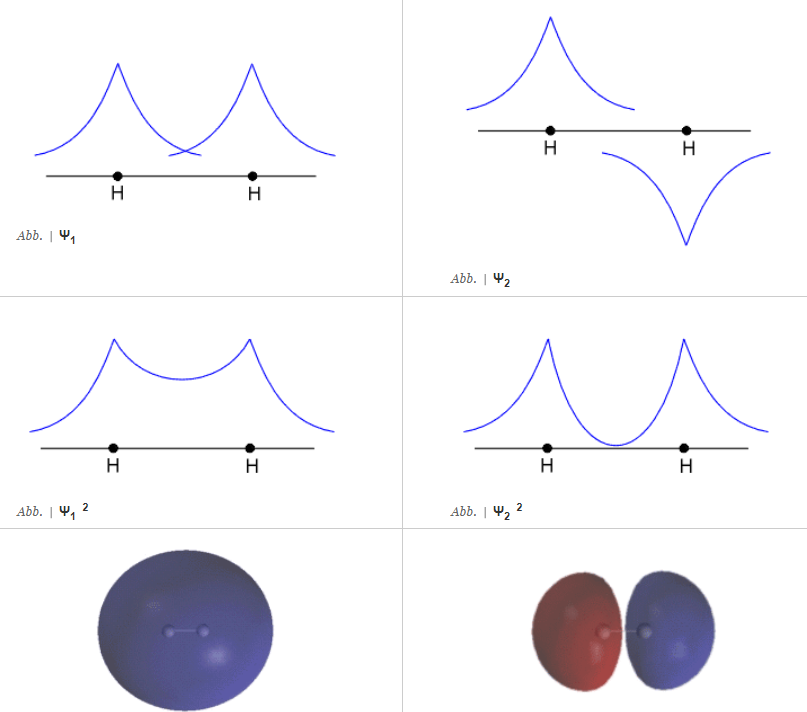
\includegraphics[width=0.7\textwidth]{orbitale.png}
\caption{Links: Bindendes Molekülorbital. Rechts: Antibindendes Molekülorbital. \cite{chemga}}
\label{fig:orbitale}
\end{figure}

\subsection{1-D Festkörper}

\begin{figure}
\centering
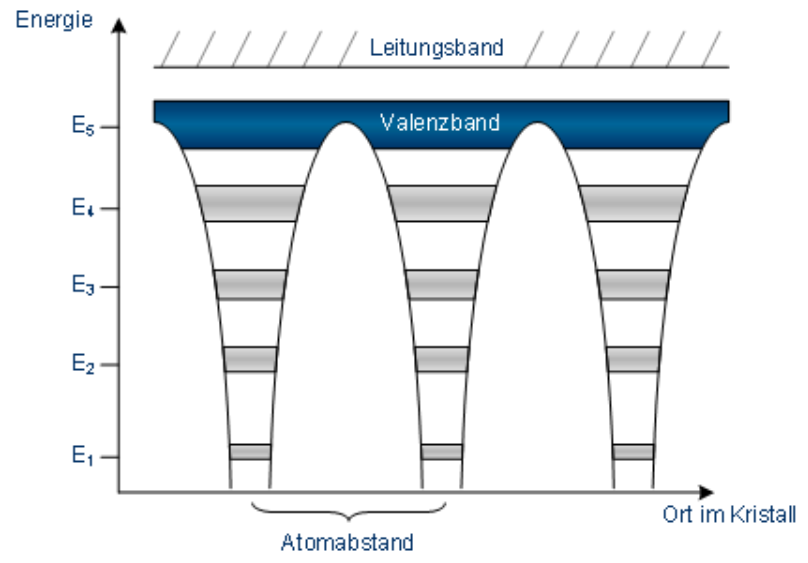
\includegraphics[width=0.6\textwidth]{baender.png}
\caption{Energiebänder der Elektronen in einem periodischen Potential eines Festkörper. \cite{halbleiter}}
\label{fig:baender}
\end{figure}

Durch die Kristallstruktur in Festkörpern beschreiben die Atome ein periodisches Potential. Die verschiedenen Energieniveaus, in
denen sich die Elektronen aufhalten können, bilden sogenannte Energiebänder. Diese entstehen aufgrund von Wechselwirkung
der Atome miteinander, sodass sich statt den diskreten Energieniveaus eines einzelnen Atoms, breitere Bereiche an
Energieniveaus ausbilden (siehe Abbildung \ref{fig:baender}).
Ein eindimensionaler Festkörper, also eine Kette von Atomen, kann mit mehreren aneinandergekoppelten Zylinderresonatoren
realisiert werden. In diesem können sich ebenfalls stehende Wellen ausbilden.

Die Wellenfunktion in so einem Festkörper wird durch die Blochfunktion beschreiben:

\begin{equation}
  \psi_k = u_k(x)e^{ikx} .
\end{equation}

Dabei gilt $u_k(x) = u_k(x+x_0)$. $u_k(x)$ ist also eine Periodizität.
